\chapter{Solution Overview}
\label{overview}

Contemporary access control models are overwhelmingly of the rule-based variety --- that
is, the policy is a set of rules in the format ``\textit{actor} is permitted to
\textit{action} on \textit{subject}''. They do not cope well with highly dynamic
systems, where strong situational awareness and ability to handle ad-hoc formed
relationships between independent agents is required. Adaptive models have been
proposed, which can handle some parts of the problem, but there is currently no
consensus on the appropriate way to control systems like smart spaces, IoT sensor
swarms, and other large-scale dynamic environments.

We are interested in a model that would have all of the following properties:

\begin{itemize}
\item \textit{Situational awareness.} The system should be context-aware by default,
able to detect situations based on low-level information, and make situation-appropriate
decisions.

\item \textit{Dynamicity.} The system should cope well with environments consisting of a
large number of agents that can appear, disappear, and form ad-hoc relationships at any
time. It should enable decomposition of the environment into logical groups, and update
immediately when availability or properties of the group members change.

\item \textit{Composability.} It should be possible to break the policy down to
functional parts and build higher levels of policy from the lower-level components.

It should also be possible to develop parts of the security policy separately, even if
they relate to the same actors or subjects. The resulting policies should be applicable
at the same time if their end results do not conflict, and there should be a way to
resolve conflicts that arise.

\item \textit{Maintainability.} The policy specification should enable good engineering
practices. Related concepts should be specified close together. Security decisions
should be made at the appropriate abstraction level. It should be easy to see which
parts of the policy are affected by a change, or which parts must be changed to achieve
the desired effect.
\end{itemize}

The idea explored in this work is to describe security situations in terms of ensembles
with attached access control decisions, have a solver element identify which components
are members of which ensembles, and apply the rules on them.

Ensemble-based architectures naturally possess the first three desired properties. They
are designed for large-scale systems composed of many independent agents, and are
suitable for highly dynamic environments. Ensemble formation depends on current context.
An ensemble is a logical group of components, so it is a decomposition of the larger
system. It can also itself be constructed from sub-ensembles, allowing composability.
Components are not limited to a single ensemble, so ensembles can overlap.

As for the fourth property, maintainability, that depends for the most part on the
design of a specification language and choice of the right abstractions. As explained in
section~\ref{background:ensembles}, declarative specification is a natural approach for
ensembles. Another notable feature we are interested in is composability on the language
level, not just on the conceptual level. Work on SCEL and DEECo is a~good inspiration
here.

\medskip

To make ensemble-based architectures applicable to the problem of dynamic access
control, we will need to tweak some of their properties.

First of all, ensemble-based systems are usually distributed and components
self-organize based on their knowledge. That approach is obviously not applicable to
access control. We will require a trusted supervisor with complete information to form
the ensembles and enforce the rules.

Another issue is beyond-control entities. Access control systems routinely deal with
independent agents beyond their control, such as humans; after all, the whole point of
an access control system is to make decisions that limit actions of beyond-control
agents. Ensemble systems, on the other hand, tend to require agent cooperation in order
to achieve their goals.

The ensembles that we use are not goal-oriented, however. There is no reason to control
actions of individual components or direct them imperatively. From the access control
point of view, component knowledge --- and indeed the ensemble structure as such --- is
purely descriptive. We can represent beyond-control entities as virtual components and
gather knowledge about them indirectly via sensors. E.g., the system can track a human's
position with an indoor positioning system and their smartphone, and can monitor room
capacity by counting incoming and outgoing door openings.

Using a central supervisor happens to help us here, too. It is a good place to store
the collected knowledge, and to perform computations that would be done on the
components in a more traditional ensemble system.

\section{Practical Example}

\begin{figure}[ht]
    \centering
    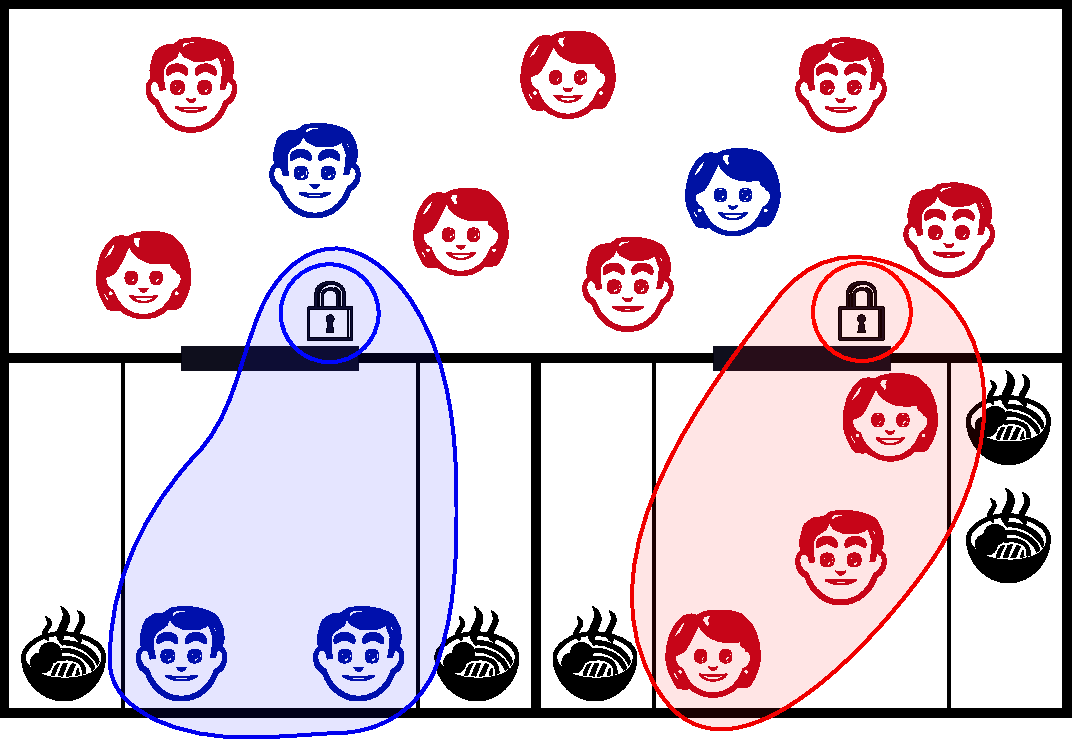
\includegraphics[width=0.68\linewidth]{img/ensemble-norequest.pdf}
    \caption{Example situation: no outstanding lunch requests}
    \label{fig:norequests}
\end{figure}

Figure~\ref{fig:norequests} illustrates a part of our running example. There are two
lunchrooms, each with six available spaces. Two people from a blue project are already
eating in the left one, and three people from a red project are eating in the right one.
The translucent shapes indicate two existing ensembles, each of which is formed around a
door lock. Membership in an ensemble grants the person a permission to open the
corresponding lock.

In the first picture, nobody is requesting access to a lunchroom. The only people
allowed to unlock the doors are those already inside, who should obviously be allowed to
leave.

\begin{figure}[h]
    \centering
    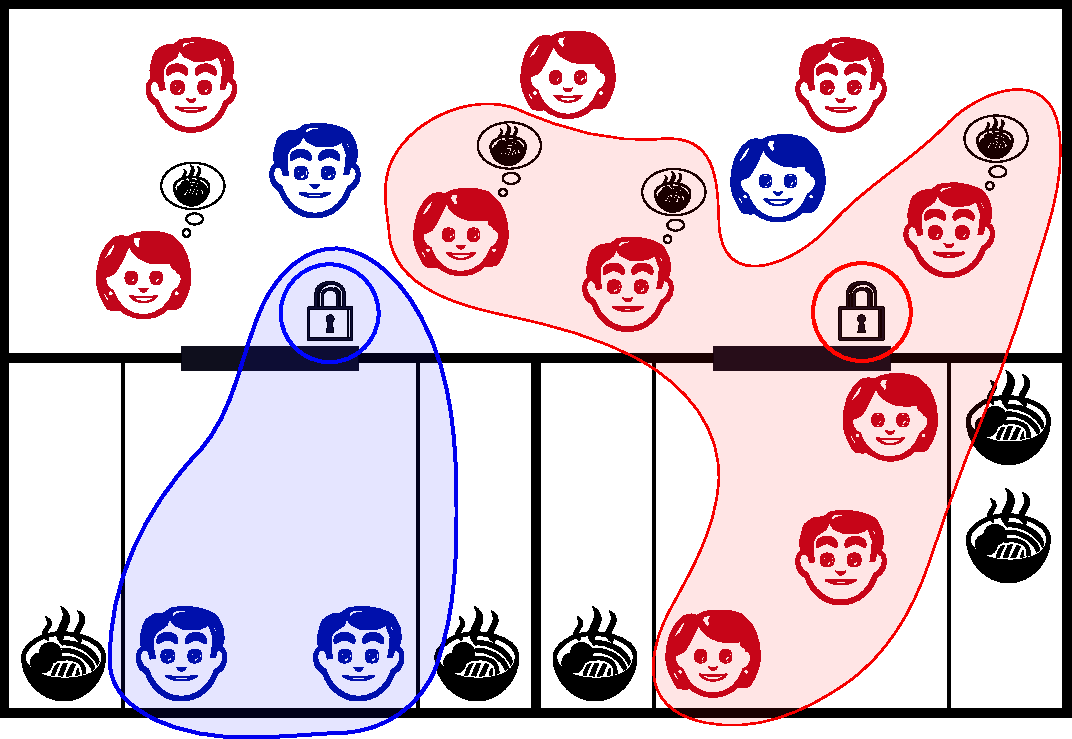
\includegraphics[width=0.68\linewidth]{img/ensemble-withrequest.pdf}
    \caption{Example situation: new lunch requests}
    \label{fig:withrequests}
\end{figure}

In picture~\ref{fig:withrequests}, four more people from the red project are hungry, as
indicated by thought bubbles. When the system is informed of this, it should allocate
lunchroom seats to the hungry people. The red ensemble extends to include three of the
hungry people --- but not the fourth, because there is no more space for them in the
lunchroom. The blue ensemble doesn't include them, because they are working on a red
project, and this would violate the constraint that people from different projects
cannot eat together.

\medskip

The example in figure~\ref{lst:pseudo} uses a pseudo-language to concisely express the
ensemble configuration, which roles exist, and what constraints limit the available
solutions. The \lstinline{allow} verbs also specify access control rules to apply on the
ensemble.

\begin{figure}[b]
    \begin{lstlisting}[style=pseudo]
ensemble Lunchroom {
    role Room = select 1 of all rooms
    role Eaters = select all of Room inhabitants
    role Requesters = select some of all hungry

    constraint {(Eaters + Requesters) must not exceed Room capacity}
    constraint {all Eaters and Requesters must have the same project}

    allow Requesters to enter Room
    allow Eaters to leave Room
}

constraint {Room from every Lunchroom must be distinct}
constraint {Requesters from every Lunchroom must be disjoint}
\end{lstlisting}
    \caption{Pseudo-code for specifying a small ensemble configuration}
    \label{lst:pseudo}
\end{figure}

The code defines an ensemble type for a single lunchroom. Three roles are defined:
\lstinline{Room} is the selected lunchroom, \lstinline{Eaters} are people already
inside, and \lstinline{Requesters} are those who are waiting for a seat. All eaters are
selected, but only some requesters. This prevents a requester from displacing someone
who is already in the room. The ensemble-local constraints ensure that we do not pick
more people than we can (which effectively only limits the number of new picks) and that
all selected people are from the same project.

Global constraints, applied over all instances of \lstinline{Lunchroom}, ensure that no
more than one ensemble is formed per room and that a single requester is not picked for
more than one lunchroom. It is important to note that ensembles are generally allowed to
overlap; without this constraint, situation on picture~\ref{fig:overlap} would be
perfectly valid. The same requester would take up space in both lunchrooms, pushing out
the hungry person in the top left.

\begin{figure}[h]
    \centering
    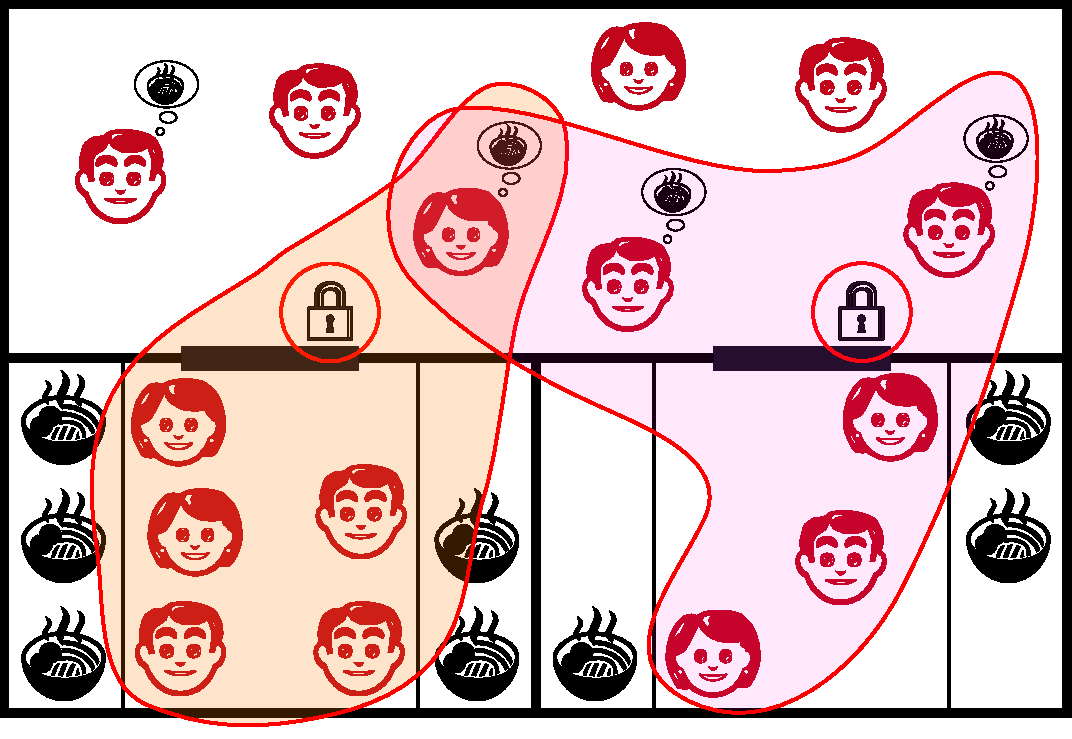
\includegraphics[width=0.68\linewidth]{img/ensemble-overlap.pdf}
    \caption{Example situation: same person is selected for both rooms}
    \label{fig:overlap}
\end{figure}

Given a definition similar to the example above, the supervisor should analyze the
current situation, choose an appropriate assignment of components to roles, and grant
the specified permissions.

\section{Goals Revisited}

There are now several open problems that must be solved in order to make the above
example actually work. There are also several more necessary features that are not shown
in the example. We can divide the goals into two distinct areas: the specification
language, and an implementation of the supervisor element. In the rest of the text, we
will call this supervisor element the \textit{solver}.

\subsection{Specification Language}

Our example uses pseudo-code to outline the desired semantics. We need a language that
is parsable by the solver and expressive enough to support all the desired features. Our
goal is to design such language and specify its semantics in detail.

Language design poses a problem on its own. It would be ideal to reuse an existing
language and only extend it to support our use-case. For this reason, we decided to
implement an internal domain-specific language (DSL). Scala~\citep{scala} was chosen as
the host language for its flexible syntax and strong typing system. Scala gives us a
repertoire of powerful language features, operators, and primitives readily available
for the DSL. We are thus free to concentrate on the specification semantics.

At its most basic, our language must allow definition of ensembles, roles within them,
and membership predicates for role inhabitants. As shown in the example, it must also be
possible to specify arbitrary constraints, applicable both locally within the ensemble
and globally over multiple ensembles. 

Next, the language must provide a way to specify when an ensemble is applicable. In our
running example, lunchrooms should only open during lunch hours. This is partially
possible with arbitrary constraints on the ensemble formation: if one of the constraints
is ``it must be lunch time'', the ensemble will simply not form at other times. However,
an ability to \textit{enforce} that a particular ensemble is formed might be useful in
certain use cases.

Many ensemble configurations can have multiple solutions. Looking back at
picture~\ref{fig:withrequests}, there is nothing in the pseudo-code specification
telling the red ensemble to find as many hungry people as it can. If the ensemble
remained the same as on picture~\ref{fig:norequests}, it would still fit all the
constraints. The specification language should thus have a way of indicating ``solution
quality'', or scoring a~given solution.

Finally, as we are interested in access control, it must be possible to attach security
decisions to the ensembles and specify when and how they apply. A~reasonable format is
RBAC-like \textit{actor-action-subject} --- it is familiar, and at the point when the
rule is applied, we have already expressed all contextual awareness by forming the
ensemble.

\subsection{Solver Implementation}

The second goal is to have a working implementation of the supervisor element. It should
process a policy specification and determine which ensembles are applicable and which
components will inhabit which roles. When the specification is ambiguous, the solver
should choose a solution that satisfies all constraints.

Given a set of components and arbitrary constraints, finding a valid role assignment can
be transformed into a constraint satisfaction problem. This would allow us to reuse an
existing constraint solver library instead of creating our own. Therefore, the solver
should be capable of converting the relevant parts of policy description into a
representation appropriate for a constraint solver.

As previously stated, some scenarios can have a method of scoring the solution quality.
The solver must be able to configure itself to either find any viable solution, or to
find a solution optimal in some variable. Furthermore, certain problems can be described
in multiple different ways, and different descriptions can have different performance
characteristics. The solver must be amenable to such tweaks, possibly even configurable
in how it explores the solution space.

And of course, after a solution is found, the solver must allow users to inspect the
solution and execute access control queries.

\subsection{Solution Novelty}

This work is a direct follow-up to the paper~\citep{isola2018}, which introduced both
the idea of using ensembles for access control, and the Scala DSL implementation which
is the basis for our framework. That implementation was presented as a proof of concept,
mainly intended for rapid prototyping. Our aim is to improve upon it in several notable
areas.

On the DSL side, our main goal is to extend, refine, and stabilize the set of available
language constructs. Each function, method, or construct should have well-defined
semantics and a~clearly stated purpose.

Another goal is to ensure that using the DSL is user-friendly and free of pitfalls. The
original code already makes good use of Scala's type system to catch many problems at
design time. We review and extend this system and clearly document the limitations of
the DSL embedding.

We ensure that the framework codebase is using good engineering practices and that it
is readable, reusable, and extendable. We provide a straightforward and efficient API
for embedding in other projects, and add a comprehensive test suite with unit tests for
each feature of the framework.

Finally, we perform detailed performance evaluation of various features of the solver
and the framework as a whole, and provide infrastructure for further measurements.
